% GNUPLOT: LaTeX picture with Postscript
\begingroup
  \makeatletter
  \providecommand\color[2][]{%
    \GenericError{(gnuplot) \space\space\space\@spaces}{%
      Package color not loaded in conjunction with
      terminal option `colourtext'%
    }{See the gnuplot documentation for explanation.%
    }{Either use 'blacktext' in gnuplot or load the package
      color.sty in LaTeX.}%
    \renewcommand\color[2][]{}%
  }%
  \providecommand\includegraphics[2][]{%
    \GenericError{(gnuplot) \space\space\space\@spaces}{%
      Package graphicx or graphics not loaded%
    }{See the gnuplot documentation for explanation.%
    }{The gnuplot epslatex terminal needs graphicx.sty or graphics.sty.}%
    \renewcommand\includegraphics[2][]{}%
  }%
  \providecommand\rotatebox[2]{#2}%
  \@ifundefined{ifGPcolor}{%
    \newif\ifGPcolor
    \GPcolortrue
  }{}%
  \@ifundefined{ifGPblacktext}{%
    \newif\ifGPblacktext
    \GPblacktexttrue
  }{}%
  % define a \g@addto@macro without @ in the name:
  \let\gplgaddtomacro\g@addto@macro
  % define empty templates for all commands taking text:
  \gdef\gplbacktext{}%
  \gdef\gplfronttext{}%
  \makeatother
  \ifGPblacktext
    % no textcolor at all
    \def\colorrgb#1{}%
    \def\colorgray#1{}%
  \else
    % gray or color?
    \ifGPcolor
      \def\colorrgb#1{\color[rgb]{#1}}%
      \def\colorgray#1{\color[gray]{#1}}%
      \expandafter\def\csname LTw\endcsname{\color{white}}%
      \expandafter\def\csname LTb\endcsname{\color{black}}%
      \expandafter\def\csname LTa\endcsname{\color{black}}%
      \expandafter\def\csname LT0\endcsname{\color[rgb]{1,0,0}}%
      \expandafter\def\csname LT1\endcsname{\color[rgb]{0,1,0}}%
      \expandafter\def\csname LT2\endcsname{\color[rgb]{0,0,1}}%
      \expandafter\def\csname LT3\endcsname{\color[rgb]{1,0,1}}%
      \expandafter\def\csname LT4\endcsname{\color[rgb]{0,1,1}}%
      \expandafter\def\csname LT5\endcsname{\color[rgb]{1,1,0}}%
      \expandafter\def\csname LT6\endcsname{\color[rgb]{0,0,0}}%
      \expandafter\def\csname LT7\endcsname{\color[rgb]{1,0.3,0}}%
      \expandafter\def\csname LT8\endcsname{\color[rgb]{0.5,0.5,0.5}}%
    \else
      % gray
      \def\colorrgb#1{\color{black}}%
      \def\colorgray#1{\color[gray]{#1}}%
      \expandafter\def\csname LTw\endcsname{\color{white}}%
      \expandafter\def\csname LTb\endcsname{\color{black}}%
      \expandafter\def\csname LTa\endcsname{\color{black}}%
      \expandafter\def\csname LT0\endcsname{\color{black}}%
      \expandafter\def\csname LT1\endcsname{\color{black}}%
      \expandafter\def\csname LT2\endcsname{\color{black}}%
      \expandafter\def\csname LT3\endcsname{\color{black}}%
      \expandafter\def\csname LT4\endcsname{\color{black}}%
      \expandafter\def\csname LT5\endcsname{\color{black}}%
      \expandafter\def\csname LT6\endcsname{\color{black}}%
      \expandafter\def\csname LT7\endcsname{\color{black}}%
      \expandafter\def\csname LT8\endcsname{\color{black}}%
    \fi
  \fi
  \setlength{\unitlength}{0.0500bp}%
  \begin{picture}(8502.00,6802.00)%
    \gplgaddtomacro\gplbacktext{%
      \csname LTb\endcsname%
      \put(784,1551){\makebox(0,0)[r]{\strut{} 94.5}}%
      \csname LTb\endcsname%
      \put(784,2010){\makebox(0,0)[r]{\strut{} 95}}%
      \csname LTb\endcsname%
      \put(784,2470){\makebox(0,0)[r]{\strut{} 95.5}}%
      \csname LTb\endcsname%
      \put(784,2930){\makebox(0,0)[r]{\strut{} 96}}%
      \csname LTb\endcsname%
      \put(784,3390){\makebox(0,0)[r]{\strut{} 96.5}}%
      \csname LTb\endcsname%
      \put(784,3850){\makebox(0,0)[r]{\strut{} 97}}%
      \csname LTb\endcsname%
      \put(784,4310){\makebox(0,0)[r]{\strut{} 97.5}}%
      \csname LTb\endcsname%
      \put(784,4770){\makebox(0,0)[r]{\strut{} 98}}%
      \csname LTb\endcsname%
      \put(784,5229){\makebox(0,0)[r]{\strut{} 98.5}}%
      \csname LTb\endcsname%
      \put(784,5689){\makebox(0,0)[r]{\strut{} 99}}%
      \csname LTb\endcsname%
      \put(784,6149){\makebox(0,0)[r]{\strut{} 99.5}}%
      \csname LTb\endcsname%
      \put(784,6609){\makebox(0,0)[r]{\strut{} 100}}%
      \csname LTb\endcsname%
      \put(880,1408){\rotatebox{-270}{\makebox(0,0)[r]{\strut{}\elu}}}%
      \csname LTb\endcsname%
      \put(1218,1408){\rotatebox{-270}{\makebox(0,0)[r]{\strut{}\selu}}}%
      \csname LTb\endcsname%
      \put(1556,1408){\rotatebox{-270}{\makebox(0,0)[r]{\strut{}\maxouta}}}%
      \csname LTb\endcsname%
      \put(1894,1408){\rotatebox{-270}{\makebox(0,0)[r]{\strut{}\mytanh}}}%
      \csname LTb\endcsname%
      \put(2231,1408){\rotatebox{-270}{\makebox(0,0)[r]{\strut{}\minsin}}}%
      \csname LTb\endcsname%
      \put(2569,1408){\rotatebox{-270}{\makebox(0,0)[r]{\strut{}\pentan}}}%
      \csname LTb\endcsname%
      \put(2907,1408){\rotatebox{-270}{\makebox(0,0)[r]{\strut{}\maxoutb}}}%
      \csname LTb\endcsname%
      \put(3245,1408){\rotatebox{-270}{\makebox(0,0)[r]{\strut{}\mysin}}}%
      \csname LTb\endcsname%
      \put(3583,1408){\rotatebox{-270}{\makebox(0,0)[r]{\strut{}\maxoutc}}}%
      \csname LTb\endcsname%
      \put(3921,1408){\rotatebox{-270}{\makebox(0,0)[r]{\strut{}\prelu}}}%
      \csname LTb\endcsname%
      \put(4259,1408){\rotatebox{-270}{\makebox(0,0)[r]{\strut{}\linear}}}%
      \csname LTb\endcsname%
      \put(4596,1408){\rotatebox{-270}{\makebox(0,0)[r]{\strut{}\lrelub}}}%
      \csname LTb\endcsname%
      \put(4934,1408){\rotatebox{-270}{\makebox(0,0)[r]{\strut{}\maxtanh}}}%
      \csname LTb\endcsname%
      \put(5272,1408){\rotatebox{-270}{\makebox(0,0)[r]{\strut{}\lrelua}}}%
      \csname LTb\endcsname%
      \put(5610,1408){\rotatebox{-270}{\makebox(0,0)[r]{\strut{}\relu}}}%
      \csname LTb\endcsname%
      \put(5948,1408){\rotatebox{-270}{\makebox(0,0)[r]{\strut{}\arctid}}}%
      \csname LTb\endcsname%
      \put(6286,1408){\rotatebox{-270}{\makebox(0,0)[r]{\strut{}\cosid}}}%
      \csname LTb\endcsname%
      \put(6623,1408){\rotatebox{-270}{\makebox(0,0)[r]{\strut{}\sigmoid}}}%
      \csname LTb\endcsname%
      \put(6961,1408){\rotatebox{-270}{\makebox(0,0)[r]{\strut{}\swish}}}%
      \csname LTb\endcsname%
      \put(7299,1408){\rotatebox{-270}{\makebox(0,0)[r]{\strut{}\maxsig}}}%
      \csname LTb\endcsname%
      \put(7637,1408){\rotatebox{-270}{\makebox(0,0)[r]{\strut{}\cube}}}%
      \put(7733,1992){\makebox(0,0)[l]{\strut{} 60}}%
      \put(7733,2569){\makebox(0,0)[l]{\strut{} 65}}%
      \put(7733,3146){\makebox(0,0)[l]{\strut{} 70}}%
      \put(7733,3723){\makebox(0,0)[l]{\strut{} 75}}%
      \put(7733,4300){\makebox(0,0)[l]{\strut{} 80}}%
      \put(7733,4878){\makebox(0,0)[l]{\strut{} 85}}%
      \put(7733,5455){\makebox(0,0)[l]{\strut{} 90}}%
      \put(7733,6032){\makebox(0,0)[l]{\strut{} 95}}%
      \put(7733,6609){\makebox(0,0)[l]{\strut{} 100}}%
      \put(128,4056){\rotatebox{-270}{\makebox(0,0){\strut{}Score}}}%
    }%
    \gplgaddtomacro\gplfronttext{%
      \csname LTb\endcsname%
      \put(6902,6466){\makebox(0,0)[r]{\strut{}\best}}%
      \csname LTb\endcsname%
      \put(6902,6306){\makebox(0,0)[r]{\strut{}\avg}}%
    }%
    \gplbacktext
    \put(0,0){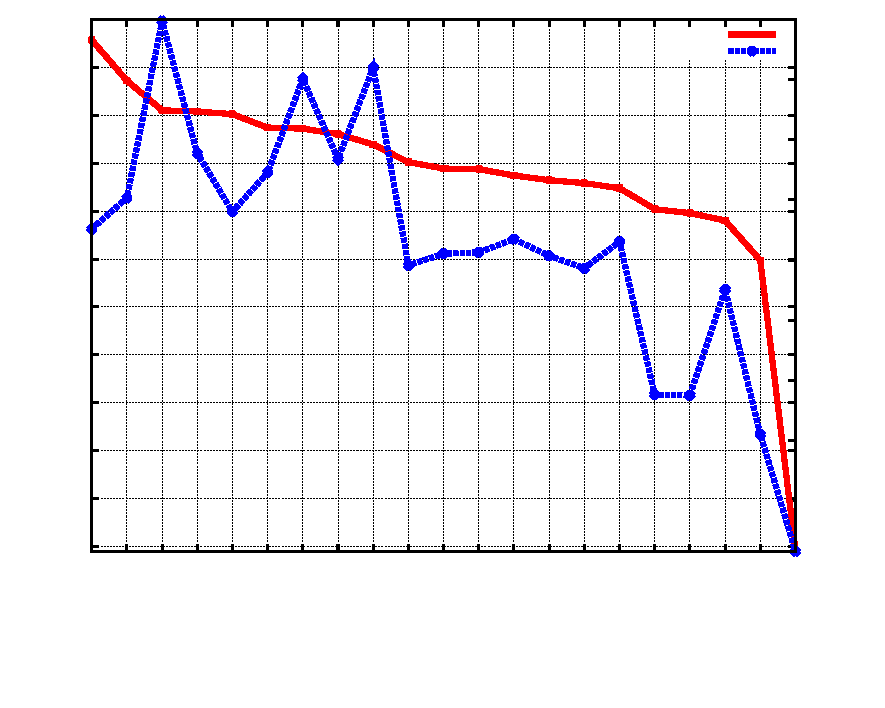
\includegraphics{plots/doc-X.pdf}}%
    \gplfronttext
  \end{picture}%
\endgroup
